\chapter{Choosing properties for property-based testing - Scott Wlaschin}
\label{sec:choosing_properties_for_testing}

\begin{quotation}
\noindent\textit{\textbf{William Yao:}}
\textit{More starting points for figuring out what properties to test.}

\vspace{\baselineskip}
\noindent\textit{Original article: \cite{choosing_properties}}
\end{quotation}

\noindent\textit{UPDATE: I did a talk on property-based testing based on these posts. \href{https://fsharpforfunandprofit.com/pbt/}{Slides and video here}.}

\vspace{\baselineskip}

\noindent In the \href{https://fsharpforfunandprofit.com/posts/property-based-testing/}{previous post}, I described the basics of property-based testing, and showed how it could save a lot of time by generating random tests.

But here's a common problem. Everyone who sees a property-based testing tool like FsCheck or QuickCheck thinks that it is amazing\ldots but when it times come to start creating your own properties, the universal complaint is: ``what properties should I use? I can't think of any!''

The goal of this post is to show some common patterns that can help you discover the properties that are applicable to your code.

\section{Categories for properties}


In my experience, many properties can be discovered by using one of the seven approaches listed below.

\begin{itemize}
\item ``Different paths, same destination'' (see \ref{sec:different_paths_same_destination})
\item ``There and back again'' (see \ref{sec:there_and_back_again})
\item ``Some things never change'' (see \ref{sec:some_things_never_change})
\item ``The more things change, the more they stay the same'' (see \ref{sec:the_more_things_change})
\item ``Solve a smaller problem first'' (see \ref{sec:solve_a_smaller_problem_first})
\item ``Hard to prove, easy to verify'' (see \ref{sec:hard_to_prove})
\item ``The test oracle'' (see \ref{sec:the_test_oracle})
\end{itemize}
This is by no means a comprehensive list, just the ones that have been most useful to me. For a different perspective, check out the list of patterns that the PEX team at Microsoft have compiled.

\subsection{``Different paths, same destination''}
\label{sec:different_paths_same_destination}

These kinds of properties are based on combining operations in different orders, but getting the same result. For example, in the diagram below, doing $X$ then $Y$ gives the same result as doing $Y$ followed by $X$ (see figure \ref{fig:choosing_properties_1}).
\begin{figure}[htbp]
 \centering
 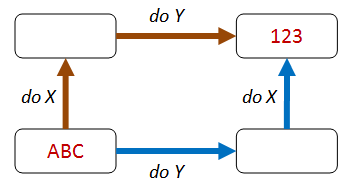
\includegraphics[width=.95\linewidth]{./pics/choosing_properties_1.png}
 \caption{Commutative Properties}
 \label{fig:choosing_properties_1}
\end{figure}
The commutative property of addition is an obvious example of this pattern. For example, the result of add 1 then add 2 is the same as the result of add 2 followed by add 1.

This pattern, generalized, can produce a wide range of useful properties. We'll see some more uses of this pattern later in this post.


\subsection{``There and back again''}
\label{sec:there_and_back_again}

These kinds of properties are based on combining an operation with its inverse, ending up with the same value you started with.

In the diagram below, doing $X$ serializes ABC to some kind of binary format, and the inverse of $X$ is some sort of deserialization that returns the same ABC value again (see figure \ref{fig:choosing_properties_2}).
\begin{figure}[htbp]
 \centering
 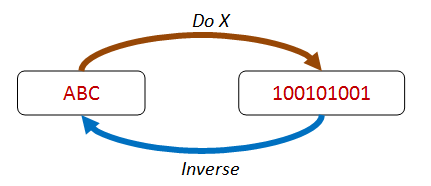
\includegraphics[width=.95\linewidth]{./pics/choosing_properties_2.png}
 \caption{Inverse Properties}
 \label{fig:choosing_properties_2}
\end{figure}
In addition to serialization/deserialization, other pairs of operations can be checked this way: \texttt{addition}/\texttt{subtraction}, \texttt{write}/\texttt{read}, \texttt{setProperty}/\texttt{getProperty}, and so on.

Other pair of functions fit this pattern too, even though they are not strict inverses, pairs such as \texttt{insert}/\texttt{contains}, \texttt{create}/\texttt{exists} , etc.



\subsection{``Some things never change''}
\label{sec:some_things_never_change}

These kinds of properties are based on an invariant that is preserved after some transformation.

In the diagram below (figure \ref{fig:choosing_properties_3}), the transform changes the order of the items, but the same four items are still present afterwards.
\begin{figure}[htbp]
 \centering
 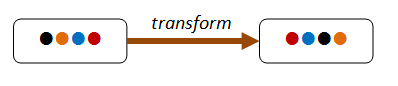
\includegraphics[width=.95\linewidth]{./pics/choosing_properties_3.png}
 \caption{Invariant Properties}
 \label{fig:choosing_properties_3}
\end{figure}
Common invariants include size of a collection (for \texttt{map} say), the contents of a collection (for sort say), the height or depth of something in proportion to size (e.g. balanced trees).

\subsection{``The more things change, the more they stay the same''}
\label{sec:the_more_things_change}

These kinds of properties are based on ``idempotence'' -- that is, doing an operation twice is the same as doing it once.

In the diagram below (figure \ref{fig:choosing_properties_4}), using distinct to filter the set returns two items, but doing distinct twice returns the same set again.
\begin{figure}[htbp]
 \centering
 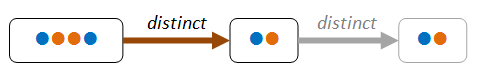
\includegraphics[width=.95\linewidth]{./pics/choosing_properties_4.png}
 \caption{Idempotent Properties}
 \label{fig:choosing_properties_4}
\end{figure}
Idempotence properties are very useful, and can be extended to things like database updates and message processing.



\subsection{``Solve a smaller problem first''}
\label{sec:solve_a_smaller_problem_first}

These kinds of properties are based on ``structural induction'' -- that is, if a large thing can be broken into smaller parts, and some property is true for these smaller parts, then you can often prove that the property is true for a large thing as well.

In the diagram below (figure \ref{fig:choosing_properties_5}), we can see that the four-item list can be partitioned into an item plus a three-item list, which in turn can be partitioned into an item plus a two-item list. If we can prove the property holds for two-item list, then we can infer that it holds for the three-item list, and for the four-item list as well.
\begin{figure}[htbp]
 \centering
 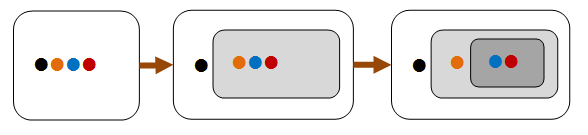
\includegraphics[width=.95\linewidth]{./pics/choosing_properties_5.png}
 \caption{Induction Properties}
 \label{fig:choosing_properties_5}
\end{figure}
Induction properties are often naturally applicable to recursive structures such as lists and trees.



\subsection{``Hard to prove, easy to verify''}
\label{sec:hard_to_prove}

Often an algorithm to find a result can be complicated, but verifying the answer is easy.

In the diagram below (figure \ref{fig:choosing_properties_6}), we can see that finding a route through a maze is hard, but checking that it works is trivial!
\begin{figure}[htbp]
 \centering
 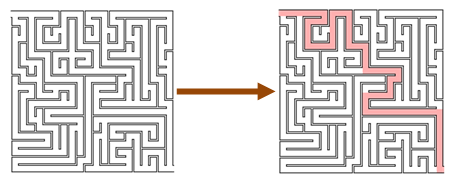
\includegraphics[width=.95\linewidth]{./pics/choosing_properties_6.png}
 \caption{Easy to Verify Properties}
 \label{fig:choosing_properties_6}
\end{figure}
Many famous problems are of this sort, such as prime number factorization. But this approach can be used for even simple problems.

For example, you might check that a string tokenizer works by just concatenating all the tokens again. The resulting string should be the same as what you started with.

\subsection{``The test oracle''}
\label{sec:the_test_oracle}

In many situations you often have an alternate version of an algorithm or process (a ``test oracle'') that you can use to check your results (figure \ref{fig:choosing_properties_7}).
\begin{figure}[htbp]
 \centering
 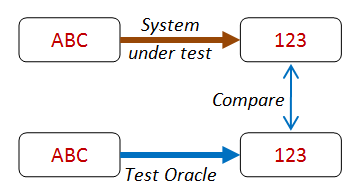
\includegraphics[width=.95\linewidth]{./pics/choosing_properties_7.png}
 \caption{Test Oracle}
 \label{fig:choosing_properties_7}
\end{figure}
For example, you might have a high-performance algorithm with optimization tweaks that you want to test. In this case, you might compare it with a brute force algorithm that is much slower but is also much easier to write correctly.

Similarly, you might compare the result of a parallel or concurrent algorithm with the result of a linear, single thread version.


\section{Putting the categories to work with some real examples}


In this section, we'll apply these categories to see if we can come up with properties for some simple functions such as ``sort a list'' and ``reverse a list''.

\subsection{``Different paths, same destination'' applied to a list sort}


Let's start with ``different paths, same destination'' and apply it to a ``list sort'' function.

Can we think of any way of combining an operation \textit{before} \texttt{List.sort}, and another operation \textit{after} \texttt{List.sort}, so that you should end up with the same result? That is, so that ``going up then across the top'' is the same as ``going across the bottom then up''.
\begin{figure}[htbp]
 \centering
 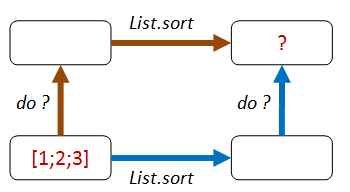
\includegraphics[width=.95\linewidth]{./pics/choosing_properties_8.png}
 \caption{List Sort Property}
 \label{fig:choosing_properties_8}
\end{figure}
How about this?

\begin{itemize}
\item \textbf{Path 1}: We add one to each element of the list, then sort.
\item \textbf{Path 2}: We sort, then add one to each element of the list.
\item Both lists should be equal.
\end{itemize}
\begin{figure}[htbp]
 \centering
 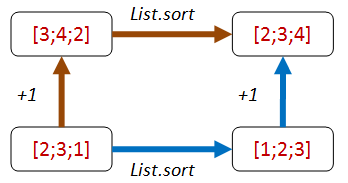
\includegraphics[width=.95\linewidth]{./pics/choosing_properties_9.png}
 \caption{List Sort Property +1}
 \label{fig:choosing_properties_9}
\end{figure}
Here's some code that implements that property:

\begin{minted}{fsharp}
let ``+1 then sort should be same as sort then +1`` sortFn aList = 
    let add1 x = x + 1
    
    let result1 = aList |> sortFn |> List.map add1
    let result2 = aList |> List.map add1 |> sortFn 
    result1 = result2

// test 
let goodSort = List.sort
Check.Quick (``+1 then sort should be same as sort then +1`` goodSort)
// Ok, passed 100 tests.
\end{minted}
Well, that works, but it also would work for a lot of other transformations too. For example, if we implemented \texttt{List.sort} as just the identity, then this property would be satisfied equally well! You can test this for yourself:

\begin{minted}{fsharp}
let badSort aList = aList
Check.Quick (``+1 then sort should be same as sort then +1`` badSort)
// Ok, passed 100 tests.
\end{minted}
The problem with this property is that it is not exploiting any of the ''sortedness``. We know that a sort will probably reorder a list, and certainly, the smallest element should be first.

How about adding an item that we know will come at the front of the list after sorting?

\begin{itemize}
\item \textbf{Path 1}: We append Int32.MinValue to the end of the list, then sort.
\item \textbf{Path 2}: We sort, then prepend Int32.MinValue to the front of the list.
\item Both lists should be equal.
\end{itemize}
\begin{figure}[htbp]
 \centering
 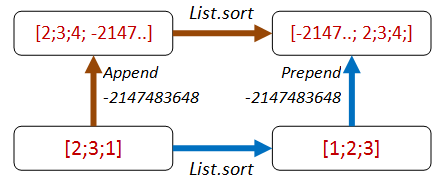
\includegraphics[width=.95\linewidth]{./pics/choosing_properties_10.png}
 \caption{List Sort Property with \texttt{Int32.MinValue}}
 \label{fig:choosing_properties_10}
\end{figure}
Here's the code:

\begin{minted}{fsharp}
let ``append minValue then sort should be same as sort then prepend minValue`` 
    sortFn aList = 
        let minValue = Int32.MinValue

        let appendThenSort = (aList @ [minValue]) |> sortFn 
        let sortThenPrepend = minValue :: (aList |> sortFn)
        appendThenSort = sortThenPrepend 

// test
Check.Quick (``append minValue then sort should be same as sort then 
    prepend minValue`` goodSort)
// Ok, passed 100 tests.
\end{minted}
The bad implementation fails now!

\begin{minted}{fsharp}
Check.Quick (``append minValue then sort should be same as sort then 
    prepend minValue`` badSort)
// Falsifiable, after 1 test (2 shrinks) 
// [0]
\end{minted}
In other words, the bad sort of \texttt{[0; minValue]} is \textit{not} the same as \texttt{[minValue; 0]}.
So that's good!

But\ldots we've got some hard coded things in there that the Enterprise Developer From Hell (\href{https://fsharpforfunandprofit.com/posts/property-based-testing/}{see previous post}) could take advantage of! The EDFH will exploit the fact that we always use \texttt{Int32.MinValue} and that we always prepend or append it to the test list.

In other words, the EDFH can identify which path we are on and have special cases for each one:

\begin{minted}{fsharp}
// The Enterprise Developer From Hell strikes again
let badSort2 aList = 
	match aList with
	| [] -> []
	| _ -> 
		let last::reversedTail = List.rev aList 
		if (last = Int32.MinValue) then
			// if min is last, move to front
			let unreversedTail = List.rev reversedTail
			last :: unreversedTail 
		else
			aList // leave alone
\end{minted}
And when we check it\ldots

\begin{minted}{fsharp}
// Oh dear, the bad implementation passes!
Check.Quick (``append minValue then sort should be same as sort then 
    prepend minValue`` badSort2)
// Ok, passed 100 tests.
\end{minted}
We could fix this by (a) picking a random number smaller than any number in the list and (b) inserting it at a random location rather than always appending it. But rather than getting too complicated, let's stop and reconsider.

An alternative approach which also exploits the ''sortedness`` is to first negate all the values, then on the path that negates \textit{after} the sort, add an extra reverse as well.
\begin{figure}[htbp]
 \centering
 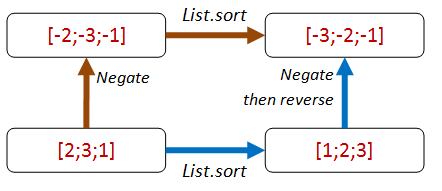
\includegraphics[width=.95\linewidth]{./pics/choosing_properties_11.png}
 \caption{List Sort Property with negate}
 \label{fig:choosing_properties_11}
\end{figure}
\begin{minted}{fsharp}
let ``negate then sort should be same as sort then negate then reverse`` 
    sortFn aList = 
        let negate x = x * -1

        let negateThenSort = aList |> List.map negate |> sortFn 
        let sortThenNegateAndReverse = aList |> sortFn |> List.map 
                negate |> List.rev
        negateThenSort = sortThenNegateAndReverse 
\end{minted}
This property is harder for the EDFH to beat because there are no magic numbers to help identify which path you are on:

\begin{minted}{fsharp}
// test
Check.Quick ( ``negate then sort should be same as sort then negate then 
    reverse`` goodSort)
// Ok, passed 100 tests.

// test
Check.Quick ( ``negate then sort should be same as sort then negate then 
    reverse``  badSort)
// Falsifiable, after 1 test (1 shrinks) 
// [1; 0]

// test
Check.Quick ( ``negate then sort should be same as sort then negate then 
    reverse``  badSort2)
// Falsifiable, after 5 tests (3 shrinks) 
// [1; 0]
\end{minted}
You might argue that we are only testing sorting for lists of integers. But the \texttt{List.sort} function is generic and knows nothing about integers per se, so I have high confidence that this property does test the core sorting logic.




\subsubsection{Applying ``different paths, same destination'' to a list
reversal function}\label{applying-different-paths-same-destination-to-a-list-reversal-function}

Ok, enough of \texttt{List.sort}. What about applying the same ideas to
the list reversal function?

We can do the same append/prepend trick:

\begin{figure}[htbp]
\centering
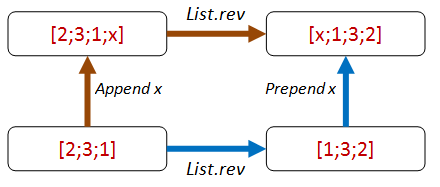
\includegraphics{pics/property_list_rev.png}
\caption{List reverse}
\end{figure}

Here's the code for the property:

\begin{minted}{fsharp}
let ``append any value then reverse should be same as reverse then prepend 
    same value`` revFn anyValue aList = 
  
	let appendThenReverse = (aList @ [anyValue]) |> revFn 
	let reverseThenPrepend = anyValue :: (aList |> revFn)
	appendThenReverse = reverseThenPrepend 
\end{minted}
Here are the test results for the correct function and for two incorrect
functions:

\begin{minted}{fsharp}
// test
let goodReverse = List.rev
Check.Quick (``append any value then reverse should be same as reverse 
    then prepend same value`` goodReverse)
// Ok, passed 100 tests.

// bad implementation fails
let badReverse aList = []
Check.Quick (``append any value then reverse should be same as reverse 
    then prepend same value`` badReverse)
// Falsifiable, after 1 test (2 shrinks) 
// true, []

// bad implementation fails
let badReverse2 aList = aList 
Check.Quick (``append any value then reverse should be same as reverse 
    then prepend same value`` badReverse2)
// Falsifiable, after 1 test (1 shrinks) 
// true, [false]
\end{minted}
You might notice something interesting here. I never specified the type
of the list. The property works with \emph{any} list.

In cases like these, FsCheck will generate random lists of bools,
strings, ints, etc.

In both failing cases, the \texttt{anyValue} is a bool. So FsCheck is
using lists of bools to start with.

Here's an exercise for you: Is this property good enough? Is there some
way that the EDFH can create an implementation that will pass?

\section{``There and back again''}\label{there-and-back-again}

Sometimes the multi-path style properties are not available or too
complicated, so let's look at some other approaches.
We'll start with properties involving inverses.

Let's start with list sorting again. Is there an inverse to sorting?
Hmmm, not really. So we'll skip sorting for now.
What about list reversal? Well, as it happens, reversal is its own
inverse!

\begin{figure}[htbp]
\centering
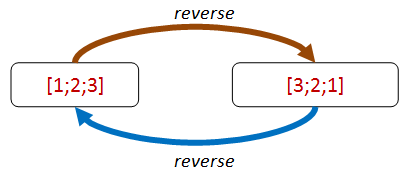
\includegraphics{pics/property_list_rev_inverse.png}
\caption{List reverse with inverse}
\end{figure}
Let's turn that into a property:

\begin{minted}{haskell}
let ``reverse then reverse should be same as original`` revFn aList = 
	let reverseThenReverse = aList |> revFn |> revFn
	reverseThenReverse = aList
\end{minted}
And it passes:

\begin{minted}{fsharp}
let goodReverse = List.rev
Check.Quick (``reverse then reverse should be same as original`` goodReverse)
// Ok, passed 100 tests.
\end{minted}
Unfortunately, a bad implementation satisfies the property too!

\begin{minted}{fsharp}
let badReverse aList = aList 
Check.Quick (``reverse then reverse should be same as original`` badReverse)
// Ok, passed 100 tests.
\end{minted}
Nevertheless, the use of properties involving inverses can be very
useful to verify that your inverse function (such as deserialization)
does indeed ``undo'' the primary function (such as serialization).

We'll see some real examples of using this in the next post.

\section{``Hard to prove, easy to
verify''}\label{hard-to-prove-easy-to-verify}

So far we've been testing properties without actually caring about the
end result of an operation. 
But of course in practice, we do care about the end result!

Now we normally can't really tell if the result is right without
duplicating the function under test. But often we can tell that the
result is \emph{wrong} quite easily. In the maze diagram from above, we
can easily check whether the path works or not.

If we are looking for the \emph{shortest} path, we might not be able to
check it, but at least we know that we have \emph{some} valid path.
This principle can be applied quite generally.

For example, let's say that we want to check whether a
\texttt{string\ split} function is working. We don't have to write a
tokenizer -- all we have to do is ensure that the tokens, when
concatenated, give us back the original string!

\begin{figure}[htbp]
\centering
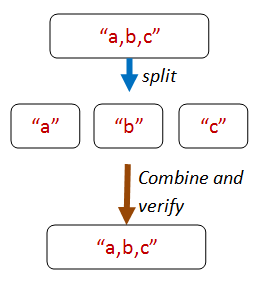
\includegraphics{pics/property_string_split.png}
\caption{String split property}
\end{figure}

Here's the core code from that property:

\begin{minted}{fsharp}
let concatWithComma s t = s + "," + t

let tokens = originalString.Split [| ',' |] 
let recombinedString = 
	// can use reduce safely because there is always at least one token
	tokens |> Array.reduce concatWithComma 

// compare the result with the original
originalString = recombinedString 
\end{minted}

But how can we create an original string? The random strings generated
by FsCheck are unlikely to contain many commas!
There are ways that you can control exactly how FsCheck generates random
data, which we'll look at later.

For now though, we'll use a trick. The trick is to let FsCheck generate
a list of random strings, and then we'll build an
\texttt{originalString} from them by concatting them together.
So here's the complete code for the property:

\begin{minted}{fsharp}
let ``concatting the elements of a string split by commas recreates the 
    original string`` aListOfStrings = 
        // helper to make a string
        let addWithComma s t = s + "," + t
        let originalString = aListOfStrings |> List.fold addWithComma ""
        
        // now for the property
        let tokens = originalString.Split [| ',' |] 
        let recombinedString = 
            // can use reduce safely because there is always at least 
            // one token
            tokens |> Array.reduce addWithComma 

        // compare the result with the original
        originalString = recombinedString 
\end{minted}
When we test this we are happy:

\begin{minted}{fsharp}
Check.Quick ``concatting the elements of a string split by commas recreates 
    the original string`` 
// Ok, passed 100 tests.
\end{minted}

\subsubsection{``Hard to prove, easy to verify'' for list
sorting}\label{hard-to-prove-easy-to-verify-for-list-sorting}

So how can we apply this principle to a sorted list? What property is
easy to verify?

The first thing that pops into my mind is that for each pair of elements
in the list, the first one will be smaller than the second.

\begin{figure}[htbp]
\centering
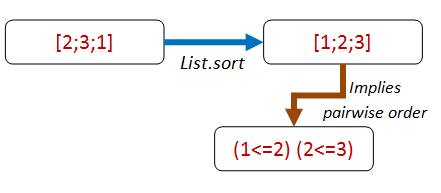
\includegraphics{pics/property_list_sort_pairwise.png}
\caption{Pairwise property}
\end{figure}

So let's make that into a property:

\begin{minted}{fsharp}
let ``adjacent pairs from a list should be ordered`` sortFn aList = 
	let pairs = aList |> sortFn |> Seq.pairwise
	pairs |> Seq.forall (fun (x,y) -> x <= y )
\end{minted}
But something funny happens when we try to check it. We get an error!

\begin{minted}{fsharp}
let goodSort = List.sort
Check.Quick (``adjacent pairs from a list should be ordered`` goodSort)
\end{minted}
\begin{verbatim}
System.Exception: Geneflect: type not handled System.IComparable
   at FsCheck.ReflectArbitrary.reflectObj@102-4.Invoke(String message)
   at Microsoft.FSharp.Core.PrintfImpl.go@523-3[b,c,d](String fmt, 
    Int32 len, FSharpFunc`2 outputChar, FSharpFunc`2 outa, b os, 
    FSharpFunc`2 finalize, FSharpList`1 args, Int32 i)
   at Microsoft.FSharp.Core.PrintfImpl.run@521[b,c,d](FSharpFunc`2 
    initialize, String fmt, Int32 len, FSharpList`1 args)
\end{verbatim}

What does
\texttt{System.Exception:\ type\ not\ handled\ System.IComparable} mean?
It means that FsCheck is trying to generate a random list, but all it
knows is that the elements must be \texttt{IComparable}. But
\texttt{IComparable} is not a type than can be instantiated, so FsCheck
throws an error.

How can we prevent this from happening? The solution is to specify a
particular type for the property, such as \texttt{int\ list}, like this:

\begin{minted}{fsharp}
let ``adjacent pairs from a list should be ordered`` sortFn 
    (aList:int list) = 
        let pairs = aList |> sortFn |> Seq.pairwise
        pairs |> Seq.forall (fun (x,y) -> x <= y )
\end{minted}
This code works now.

\begin{minted}{fsharp}
let goodSort = List.sort
Check.Quick (``adjacent pairs from a list should be ordered`` goodSort)
// Ok, passed 100 tests.
\end{minted}
Note that even though the property has been constrained, the property is
still a very general one. We could have used \texttt{string\ list}
instead, for example, and it would work just the same.

\begin{minted}{fsharp}
let ``adjacent pairs from a string list should be ordered`` sortFn 
    (aList:string list) = 
        let pairs = aList |> sortFn |> Seq.pairwise
        pairs |> Seq.forall (fun (x,y) -> x <= y )

Check.Quick (``adjacent pairs from a string list should be ordered`` goodSort)
// Ok, passed 100 tests.
\end{minted}
\textbf{TIP: If FsCheck throws ``type not handled'', add explicit type
constraints to your property}

Are we done now? No! One problem with this property is that it doesn't
catch malicious implementations by the EDFH.

\begin{minted}{fsharp}
// bad implementation passes
let badSort aList = []
Check.Quick (``adjacent pairs from a list should be ordered`` badSort)
// Ok, passed 100 tests.
\end{minted}
Is it a surprise to you that a silly implementation also works?
Hmmm. That tells us that there must be some property \emph{other than
pairwise ordering} associated with sorting that we've overlooked. What
are we missing here?

This is a good example of how doing property-based testing can lead to
insights about design. We thought we knew what sorting meant, but we're
being forced to be a bit stricter in our definition.
As it happens, we'll fix this particular problem by using the next
principle!

\section{``Some things never
change''}\label{some-things-never-change}

A useful kind of property is based on an invariant that is preserved
after some transformation, such as preserving length or contents.

They are not normally sufficient in themselves to ensure a correct
implementation, but they \emph{do} often act as a counter-check to more
general properties. 
For example, in \href{https://fsharpforfunandprofit.com/posts/property-based-testing/}{the previous
post}, we created commutative and associative properties for addition,
but then noticed that simply having an implementation that returned zero
would satisfy them just as well! It was only when we added
\texttt{x\ +\ 0\ =\ x} as a property that we could eliminate that
particular malicious implementation.

And in the ``list sort'' example above, we could satisfy the ``pairwise
ordered'' property with a function that just returned an empty list! How
could we fix that?
Our first attempt might be to check the length of the sorted list. If
the lengths are different, then the sort function obviously cheated!

\begin{minted}{fsharp}
let ``sort should have same length as original`` sortFn (aList:int list) = 
	let sorted = aList |> sortFn 
	List.length sorted = List.length aList
\end{minted}
We check it and it works:

\begin{minted}{fsharp}
let goodSort = List.sort
Check.Quick (``sort should have same length as original`` goodSort )
// Ok, passed 100 tests.
\end{minted}
And yes, the bad implementation fails:

\begin{minted}{fsharp}
let badSort aList = []
Check.Quick (``sort should have same length as original`` badSort )
// Falsifiable, after 1 test (1 shrink) 
// [0]
\end{minted}
Unfortunately, the BDFH is not defeated and can come up with another
compliant implementation! Just repeat the first element N times!

\begin{minted}{fsharp}
// bad implementation has same length
let badSort2 aList = 
	match aList with 
	| [] -> []
	| head::_ -> List.replicate (List.length aList) head 

// for example 
// badSort2 [1;2;3] => [1;1;1]
\end{minted}
Now when we test this, it passes:

\begin{minted}{fsharp}
Check.Quick (``sort should have same length as original`` badSort2)
// Ok, passed 100 tests.
\end{minted}
What's more, it also satisfies the pairwise property too!

\begin{minted}{fsharp}
Check.Quick (``adjacent pairs from a list should be ordered`` badSort2)
// Ok, passed 100 tests.
\end{minted}


\subsection{Sort invariant - 2nd
attempt}\label{sort-invariant---2nd-attempt}

So now we have to try again. What is the difference between the real
result \texttt{{[}1;2;3{]}} and the fake result \texttt{{[}1;1;1{]}}?

Answer: the fake result is throwing away data. The real result always
contains the same contents as the original list, but just in a different
order.

\begin{figure}[htbp]
\centering
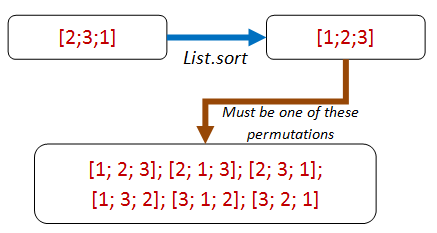
\includegraphics{pics/property_list_sort_permutation.png}
\caption{Permutation property}
\end{figure}

That leads us to a new property: a sorted list is always a permutation
of the original list. Aha! Let's write the property in terms of
permutations now:

\begin{minted}{fsharp}
let ``a sorted list is always a permutation of the original list`` 
    sortFn (aList:int list) = 
        let sorted = aList |> sortFn 
        let permutationsOfOriginalList = permutations aList 

        // the sorted list must be in the seq of permutations
        permutationsOfOriginalList 
        |> Seq.exists (fun permutation -> permutation = sorted) 
\end{minted}
Great, now all we need is a permutation function.
Let's head over to StackOverflow and \sout{steal}
\href{http://stackoverflow.com/a/4610704/1136133}{borrow an
implementation}. Here it is:

\begin{minted}{fsharp}
/// given aList and anElement to insert,
/// generate all possible lists with anElement 
/// inserted into aList 
let rec insertElement anElement aList =
	// From http://stackoverflow.com/a/4610704/1136133
	seq { 
		match aList with
		// empty returns a singleton
		| [] -> yield [anElement] 
		// not empty? 
		| first::rest ->
			// return anElement prepended to the list
			yield anElement::aList
			// also return first prepended to all the sublists
			for sublist in insertElement anElement rest do
				yield first::sublist
		}

/// Given a list, return all permutations of it
let rec permutations aList =
	seq { 
		match aList with
		| [] -> yield []
		| first::rest ->
			// for each sub-permutation, 
			// return the first inserted into it somewhere
			for sublist in permutations rest do
				yield! insertElement first sublist
		}
\end{minted}
Some quick interactive tests confirm that it works as expected:

\begin{minted}{fsharp}
permutations ['a';'b';'c'] |> Seq.toList
// [['a'; 'b'; 'c']; ['b'; 'a'; 'c']; ['b'; 'c'; 'a']; ['a'; 'c'; 'b'];
// ['c'; 'a'; 'b']; ['c'; 'b'; 'a']]

permutations ['a';'b';'c';'d'] |> Seq.toList
// [['a'; 'b'; 'c'; 'd']; ['b'; 'a'; 'c'; 'd']; ['b'; 'c'; 'a'; 'd'];
// ['b'; 'c'; 'd'; 'a']; ['a'; 'c'; 'b'; 'd']; ['c'; 'a'; 'b'; 'd'];
// ['c'; 'b'; 'a'; 'd']; ['c'; 'b'; 'd'; 'a']; ['a'; 'c'; 'd'; 'b'];
// ['c'; 'a'; 'd'; 'b']; ['c'; 'd'; 'a'; 'b']; ['c'; 'd'; 'b'; 'a'];
// ['a'; 'b'; 'd'; 'c']; ['b'; 'a'; 'd'; 'c']; ['b'; 'd'; 'a'; 'c'];
// ['b'; 'd'; 'c'; 'a']; ['a'; 'd'; 'b'; 'c']; ['d'; 'a'; 'b'; 'c'];
// ['d'; 'b'; 'a'; 'c']; ['d'; 'b'; 'c'; 'a']; ['a'; 'd'; 'c'; 'b'];
// ['d'; 'a'; 'c'; 'b']; ['d'; 'c'; 'a'; 'b']; ['d'; 'c'; 'b'; 'a']]

permutations [3;3] |> Seq.toList
// [[3; 3]; [3; 3]]
\end{minted}
Excellent! Now let's run FsCheck:

\begin{minted}{fsharp}
Check.Quick (``a sorted list is always a permutation of the original 
    list`` goodSort)
\end{minted}
Hmmm. That's funny, nothing seems to be happening. And my CPU is maxing
out for some reason. What's going on?

What's going on is that you are going to be sitting there for a long
time! If you are following along at home, I suggest you right-click and
cancel the interactive session now.
The innocent looking \texttt{permutations} is really \emph{really} slow
for any normal sized list. For example, a list of just 10 items has
3,628,800 permutations. While with 20 items, you are getting to
astronomical numbers.
And of course, FsCheck will be doing hundreds of these tests! So this
leads to an important tip:

\textbf{TIP: Make sure your property checks are very fast. You will be
running them a LOT!}

We've already seen that even in the best case, FsCheck will evaluate the
property 100 times. And if shrinking is needed, even more. So make sure
your tests are fast to run!
But what happens if you are dealing with real systems such as databases,
networks, or other slow dependencies?

In his (highly recommended) \href{http://vimeo.com/68383317}{video on
using QuickCheck}, John Hughes tells of when his team was trying to
detect flaws in a distributed data store that could be caused by network
partitions and node failures.
Of course, killing real nodes thousands of times was too slow, so they
extracted the core logic into a virtual model, and tested that instead.
As a result, the code was \emph{later refactored} to make this kind of
testing easier. In other words, property-based testing influenced the
design of the code, just as TDD would.

\subsection{Sort invariant - 3rd
attempt}\label{sort-invariant---3rd-attempt}

Ok, so we can't use permutations by just looping through them. So let's
use the same idea but write a function that is specific for this case, a
\texttt{isPermutationOf} function.

\begin{minted}{fsharp}
let ``a sorted list has same contents as the original list`` sortFn 
    (aList:int list) = 
        let sorted = aList |> sortFn 
        isPermutationOf aList sorted
\end{minted}
Here's the code for \texttt{isPermutationOf} and its associated helper
functions:

\begin{minted}{fsharp}
/// Given an element and a list, and other elements previously 
/// skipped,
/// return a new list without the specified element.
/// If not found, return None
let rec withoutElementRec anElement aList skipped = 
	match aList with
	| [] -> None
	| head::tail when anElement = head -> 
		// matched, so create a new list from the skipped and 
		// the remaining
		// and return it
		let skipped' = List.rev skipped
		Some (skipped' @ tail)
	| head::tail  -> 
		// no match, so prepend head to the skipped and recurse 
		let skipped' = head :: skipped
		withoutElementRec anElement tail skipped' 

/// Given an element and a list
/// return a new list without the specified element.
/// If not found, return None
let withoutElement x aList = 
	withoutElementRec x aList [] 

/// Given two lists, return true if they have the same contents
/// regardless of order
let rec isPermutationOf list1 list2 = 
	match list1 with
	| [] -> List.isEmpty list2 // if both empty, true
	| h1::t1 -> 
		match withoutElement h1 list2 with
		| None -> false
		| Some t2 -> 
			isPermutationOf t1 t2
\end{minted}

Let's try the test again. And yes, this time it completes before the
heat death of the universe.

\begin{minted}{fsharp}
Check.Quick (``a sorted list has same contents as the original list``  
    goodSort)
// Ok, passed 100 tests.
\end{minted}
What's also great is that the malicious implementation now fails to
satisfy this property!

\begin{minted}{fsharp}
Check.Quick (``a sorted list has same contents as the original list``  
    badSort2)
// Falsifiable, after 2 tests (5 shrinks) 
// [1; 0]
\end{minted}
In fact, these two properties,
\texttt{adjacent\ pairs\ from\ a\ list\ should\ be\ ordered} and
\texttt{a\ sorted\ list\ has\ same\ contents\ as\ the\ original\ list}
should indeed ensure that any implementation is correct.

\section{Sidebar: Combining
properties}\label{sidebar-combining-properties}

Just above, we noted that there were \emph{two} properties needed to
define the ``is sorted'' property. It would be nice if we could combine
them into one property \texttt{is\ sorted} so that we can have a single
test.

Well, of course we can always merge the two sets of code into one
function, but it's preferable to keep functions as small as possible.
Furthermore, a property like \texttt{has\ same\ contents} might be
reusable in other contexts as well.
What we want then, is an equivalent to \texttt{AND} and \texttt{OR} that
is designed to work with properties.

FsCheck to the rescue! There are built in operators to combine
properties: \texttt{.\&.} for \texttt{AND} and \texttt{.\textbar{}.} for
\texttt{OR}.
Here is an example of them in use:

\begin{minted}{fsharp}
let ``list is sorted``sortFn (aList:int list) = 
	let prop1 = ``adjacent pairs from a list should be ordered`` sortFn 
            aList 
	let prop2 = ``a sorted list has same contents as the original list`` 
            sortFn aList 
	prop1 .&. prop2 
\end{minted}
When we test the combined property with a good implementation of
\texttt{sort}, everything works as expected.

\begin{minted}{fsharp}
let goodSort = List.sort
Check.Quick (``list is sorted`` goodSort )
// Ok, passed 100 tests.
\end{minted}
And if we test a bad implementation, the combined property fails as
well.

\begin{minted}{fsharp}
let badSort aList = []
Check.Quick (``list is sorted`` badSort )
// Falsifiable, after 1 test (0 shrinks) 
// [0]
\end{minted}
But there's a problem now. Which of the two properties failed?

What we would like to do is add a ``label'' to each property so that we
can tell them apart. In FsCheck, this is done with the
\texttt{\textbar{}@} operator:

\begin{minted}{fsharp}
let ``list is sorted (labelled)``sortFn (aList:int list) = 
    let prop1 = ``adjacent pairs from a list should be ordered`` sortFn 
            aList 
                |@ "adjacent pairs from a list should be ordered"
    let prop2 = ``a sorted list has same contents as the original list`` 
            sortFn aList 
                |@ "a sorted list has same contents as the original list"
    prop1 .&. prop2 
\end{minted}
And now, when we test with the bad sort, we get a message
\texttt{Label\ of\ failing\ property:\ a\ sorted\ list\ has\ same\ contents\ as\ the\ 
    original\ list}:

\begin{minted}{fsharp}
Check.Quick (``list is sorted (labelled)`` badSort )
// Falsifiable, after 1 test (2 shrinks)
// Label of failing property: a sorted list has same contents as the 
// original list
// [0]
\end{minted}
For more on these operators,
\href{https://fscheck.github.io/FsCheck/Properties.html\#And-Or-and-Labels}{see
the FsCheck documentation under ``And, Or and Labels''}.

And now, back to the property-divising strategies.

\section{``Solving a smaller
problem''}\label{solving-a-smaller-problem}

Sometimes you have a recursive data structure or a recursive problem. In
these cases, you can often find a property that is true of a smaller
part.

For example, for a sort, we could say something like:

\begin{verbatim}
A list is sorted if:
* The first element is smaller (or equal to) the second.
* The rest of the elements after the first element are also sorted.
\end{verbatim}

Here is that logic expressed in code:

\begin{minted}{fsharp}
let rec ``First element is <= than second, and tail is also sorted`` 
        sortFn (aList:int list) = 
    let sortedList = aList |> sortFn 
    match sortedList with
    | [] -> true
    | [first] -> true
    | [first;second] -> 
        first <= second
    | first::second::tail -> 
        first <= second &&
        let subList = second::tail 
        ``First element is <= than second, and tail is also sorted`` 
            sortFn subList  
\end{minted}
This property is satisfied by the real sort function:

\begin{minted}{fsharp}
let goodSort = List.sort
Check.Quick (``First element is <= than second, and tail is also sorted`` 
    goodSort )
// Ok, passed 100 tests.
\end{minted}
But unfortunately, just like previous examples, the malicious
implementations also pass.

\begin{minted}{fsharp}
let badSort aList = []
Check.Quick (``First element is <= than second, and tail is also sorted`` 
    badSort )
// Ok, passed 100 tests.

let badSort2 aList = 
	match aList with 
	| [] -> []
	| head::_ -> List.replicate (List.length aList) head 

Check.Quick (``First element is <= than second, and tail is also sorted`` 
    badSort2)
// Ok, passed 100 tests.
\end{minted}
So as before, we'll need another property (such as the
\texttt{has\ same\ contents} invariant) to ensure that the code is
correct.

If you do have a recursive data structure, then try looking for
recursive properties. They are pretty obvious and low hanging, when you
get the hang of it.

\section{Is the EDFH really a
problem?}\label{is-the-edfh-really-a-problem}

In the last few examples, I've noted that trivial but wrong
implementations often satisfy the properties as well as good
implementations.
But should we \emph{really} spend time worrying about this? I mean, if
we ever really released a sort algorithm that just duplicated the first
element it would be obvious immediately, surely?

So yes, it's true that truly malicious implementations are unlikely to
be a problem. On the other hand, you should think of property-based
testing not as a \emph{testing} process, but as a \emph{design} process
-- a technique that helps you clarify what your system is really trying
to do. And if a key aspect of your design is satisfied with just a
simple implementation, then perhaps there is something you have
overlooked -- something that, when you discover it, will make your
design both clearer and more robust.

\section{``The more things change, the more they stay the
same''}\label{the-more-things-change-the-more-they-stay-the-same}

Our next type of property is ``idempotence''. Idempotence simply means
that doing something twice is the same as doing it once. If I tell you
to ``sit down'' and then tell you to ``sit down'' again, the second
command has no effect.

Idempotence is
\href{https://queue.acm.org/detail.cfm?id=2187821}{essential for
reliable systems} and is
\href{http://soapatterns.org/design_patterns/idempotent_capability}{a
key aspect of service oriented} and message-based architectures.
If you are designing these kinds of real-world systems it is well worth
ensuring that your requests and processes are idempotent.
I won't go too much into this right now, but let's look at two simple
examples.

First, our old friend \texttt{sort} is idempotent (ignoring stability)
while \texttt{reverse} is not, obviously.

\begin{minted}{fsharp}
let ``sorting twice gives the same result as sorting once`` sortFn 
    (aList:int list) =
        let sortedOnce = aList |> sortFn 
        let sortedTwice = aList |> sortFn |> sortFn 
        sortedOnce = sortedTwice

// test
let goodSort = List.sort
Check.Quick (``sorting twice gives the same result as sorting once`` 
    goodSort )
// Ok, passed 100 tests.
\end{minted}
In general, any kind of query should be idempotent, or to put it another
way:
\href{https://en.wikipedia.org/wiki/Command\%E2\%80\%93query_separation}{``asking
a question should not change the answer''}.
In the real world, this may not be the case. A simple query on a
datastore run at different times may give different results.

Here's a quick demonstration.
First we'll create a \texttt{NonIdempotentService} that gives different
results on each query.

\begin{minted}{fsharp}
type NonIdempotentService() =
    let mutable data = 0
    member this.Get() = 
        data
    member this.Set value = 
        data <- value

let ``querying NonIdempotentService after update gives the same result`` 
    value1 value2 =
        let service = NonIdempotentService()
        service.Set value1

        // first GET 
        let get1 = service.Get()

        // another task updates the data store
        service.Set value2

        // second GET called just like first time
        let get2 = service.Get() 
        get1 = get2 
\end{minted}
But if we test it now, we find that it does not satisfy the required
idempotence property:

\begin{minted}{fsharp}
Check.Quick ``querying NonIdempotentService after update gives the same result``
// Falsifiable, after 2 tests
\end{minted}
As an alternative, we can create a (crude) \texttt{IdempotentService}
that requires a timestamp for each transaction. In this design, multiple
GETs using the same timestamp will always retrieve the same data.

\begin{minted}{fsharp}
type IdempotentService() =
    let mutable data = Map.empty
    member this.GetAsOf (dt:DateTime) = 
        data |> Map.find dt
    member this.SetAsOf (dt:DateTime) value = 
        data <- data |> Map.add dt value

let ``querying IdempotentService after update gives the same result`` 
    value1 value2 =
        let service = IdempotentService()
        let dt1 = DateTime.Now.AddMinutes(-1.0)
        service.SetAsOf dt1 value1

        // first GET 
        let get1 = service.GetAsOf dt1 

        // another task updates the data store
        let dt2 = DateTime.Now
        service.SetAsOf dt2 value2

        // second GET called just like first time
        let get2 = service.GetAsOf dt1 
        get1 = get2 
\end{minted}
And this one works:

\begin{minted}{fsharp}
Check.Quick ``querying IdempotentService after update gives the same result``
// Ok, passed 100 tests.
\end{minted}
So, if you are building a REST GET handler or a database query service,
and you want idempotence, you should consider using techniques such as
etags, ``as-of'' times, date ranges, etc.
If you need tips on how to do this, searching for
\href{http://blog.jonathanoliver.com/idempotency-patterns/}{idempotency
patterns} will turn up some good results.

\section{``Two heads are better than
one''}\label{two-heads-are-better-than-one}

And finally, last but not least, we come to the ``test oracle''. A test
oracle is simply an alternative implementation that gives the right
answer, and that you can check your results against.

Often the test oracle implementation is not suitable for production --
it's too slow, or it doesn't parallelize, or it's
\href{https://xkcd.com/1026/}{too poetic}, etc., but that doesn't stop
it being very useful for testing.
So for ``list sort'', there are many simple but slow implementations
around. For example, here's a quick implementation of insertion sort:

\begin{minted}{fsharp}
module InsertionSort = 
	
	// Insert a new element into a list by looping over the list.
	// As soon as you find a larger element, insert in front of it
	let rec insert newElem list = 
		match list with 
		| head::tail when newElem > head -> 
			head :: insert newElem tail
		| other -> // including empty list
			newElem :: other 

	// Sorts a list by inserting the head into the rest of the list 
	// after the rest have been sorted
	let rec sort list = 
		match list with
		| []   -> []
		| head::tail -> 
			insert head (sort tail)

	// test
	// insertionSort [5;3;2;1;1]
\end{minted}
With this in place, we can write a property that tests the result
against insertion sort.

\begin{minted}{fsharp}
let ``sort should give same result as insertion sort`` sortFn (aList:int list) = 
	let sorted1 = aList |> sortFn 
	let sorted2 = aList |> InsertionSort.sort
	sorted1 = sorted2 
\end{minted}
When we test the good sort, it works. Good!

\begin{minted}{fsharp}
let goodSort = List.sort
Check.Quick (``sort should give same result as insertion sort`` goodSort)
// Ok, passed 100 tests.
\end{minted}
And when we test a bad sort, it doesn't. Even better!

\begin{minted}{fsharp}
let badSort aList = aList 
Check.Quick (``sort should give same result as insertion sort`` badSort)
// Falsifiable, after 4 tests (6 shrinks) 
// [1; 0]
\end{minted}


\section{Generating Roman numerals in two different
ways}\label{generating-roman-numerals-in-two-different-ways}

We can also use the test oracle approach to cross-check two different
implementations when you're not sure that \emph{either} implementation
is right!

For example, in my post \href{/posts/roman-numeral-kata/}{``Commentary
on `Roman Numerals Kata with Commentary'\,''} I came up with two
completely different algorithms for generating Roman Numerals. Can we
compare them to each other and test them both in one fell swoop?
The first algorithm was based on understanding that Roman numerals were
based on tallying, leading to this simple code:

\begin{minted}{fsharp}
let arabicToRomanUsingTallying arabic = 
   (String.replicate arabic "I")
	.Replace("IIIII","V")
	.Replace("VV","X")
	.Replace("XXXXX","L")
	.Replace("LL","C")
	.Replace("CCCCC","D")
	.Replace("DD","M")
	// optional substitutions
	.Replace("IIII","IV")
	.Replace("VIV","IX")
	.Replace("XXXX","XL")
	.Replace("LXL","XC")
	.Replace("CCCC","CD")
	.Replace("DCD","CM")
\end{minted}
Another way to think about Roman numerals is to imagine an abacus. Each
wire has four ``unit'' beads and one ``five'' bead.
This leads to the so-called ``bi-quinary'' approach:

\begin{minted}{fsharp}
let biQuinaryDigits place (unit,five,ten) arabic =
  let digit =  arabic % (10*place) / place
  match digit with
  | 0 -> ""
  | 1 -> unit
  | 2 -> unit + unit
  | 3 -> unit + unit + unit
  | 4 -> unit + five // changed to be one less than five 
  | 5 -> five
  | 6 -> five + unit
  | 7 -> five + unit + unit
  | 8 -> five + unit + unit + unit
  | 9 -> unit + ten  // changed to be one less than ten
  | _ -> failwith "Expected 0-9 only"

let arabicToRomanUsingBiQuinary arabic = 
  let units = biQuinaryDigits 1 ("I","V","X") arabic
  let tens = biQuinaryDigits 10 ("X","L","C") arabic
  let hundreds = biQuinaryDigits 100 ("C","D","M") arabic
  let thousands = biQuinaryDigits 1000 ("M","?","?") arabic
  thousands + hundreds + tens + units
\end{minted}
We now have two completely different algorithms, and we can cross-check
them with each other to see if they give the same result.

\begin{minted}{fsharp}
let ``biquinary should give same result as tallying`` arabic = 
	let tallyResult = arabicToRomanUsingTallying arabic 
	let biquinaryResult = arabicToRomanUsingBiQuinary arabic 
	tallyResult = biquinaryResult 
\end{minted}
But if we try running this code, we get a
\texttt{ArgumentException:\ The\ input\ must\ be\ non-negative} due to
the \texttt{String.replicate} call.

\begin{minted}{fsharp}
Check.Quick ``biquinary should give same result as tallying``
// ArgumentException: The input must be non-negative.
\end{minted}
So we need to only include inputs that are positive. We also need to
exclude numbers that are greater than 4000, say, since the algorithms
break down there too.
How can we implement this filter?

We saw in the previous post that we could use preconditions. But for
this example, we'll try something different and change the generator.
First we'll define a \emph{new} arbitrary integer called
\texttt{arabicNumber} which is filtered as we want (an ``arbitrary'' is
a combination of a generator algorithm and a shrinker algorithm, as
described in the previous post).

\begin{minted}{fsharp}
let arabicNumber = Arb.Default.Int32() |> Arb.filter (fun i -> i > 0 
    && i <= 4000) 
\end{minted}
Next, we create a new property \emph{which is constrained to only use
``arabicNumber''} by using the \texttt{Prop.forAll} helper.

We'll give the property the rather clever name of ``for all values of
arabicNumber, biquinary should give same result as tallying''.

\begin{minted}{fsharp}
let ``for all values of arabicNumber biquinary should give same result 
    as tallying`` = 
        Prop.forAll arabicNumber ``biquinary should give same result as 
            tallying`` 
\end{minted}
Now finally, we can do the cross-check test:

\begin{minted}{fsharp}
Check.Quick ``for all values of arabicNumber biquinary should give same 
    result as tallying``
// Ok, passed 100 tests.
\end{minted}
And we're good! Both algorithms work correctly, it seems.

\section{``Model-based'' testing}\label{model-based-testing}

``Model-based'' testing, which we will discuss in more detail in a later
post, is a variant on having a test oracle.
The way it works is that, in parallel with your (complex) system under
test, you create a simplified model.
Then, when you do something to the system under test, you do the same
(but simplified) thing to your model.
At the end, you compare your model's state with the state of the system
under test. If they are the same, you're done. If not, either your SUT
is buggy or your model is wrong and you have to start over!

\section{Interlude: A game based on finding
properties}\label{interlude-a-game-based-on-finding-properties}

With that, we have come to the end of the various property categories.
We'll go over them one more time in a minute -- but first, an interlude.

If you sometimes feel that trying to find properties is a mental
challenge, you're not alone. Would it help to pretend that it is a game?
As it happens, there \emph{is} a game based on property-based testing.
It's called \href{http://boardgamegeek.com/boardgame/6830/zendo}{Zendo}
and it involves placing sets of objects (such as plastic pyramids) on a
table, such that each layout conforms to a pattern -- a rule -- or as we
would now say, \emph{a property}!.

The other players then have to guess what the rule (property) is, based
on what they can see.
Here's a picture of a Zendo game in progress (figure \ref{fig:zendo}).

\begin{figure}[htbp]
\centering
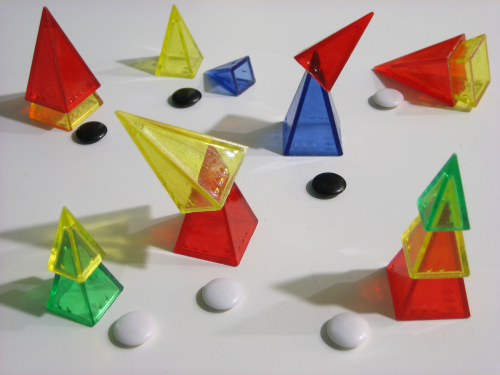
\includegraphics{pics/zendo1.png}
\caption{Zendo}
\label{fig:zendo}
\end{figure}

The white stones mean the property has been satisfied, while black
stones mean failure. Can you guess the rule here? I'm going to guess
that it's something like ``a set must have a yellow pyramid that's not
touching the ground''.

Alright, I suppose Zendo wasn't really inspired by property-based
testing, but it is a fun game, and it has even been known to make an
appearance at
\href{http://blog.fogus.me/2014/10/23/games-of-interest-zendo/}{programming
conferences}.
If you want to learn more about Zendo,
\href{http://www.looneylabs.com/rules/zendo}{the rules are here}.

\section{Applying the categories one more
time}\label{applying-the-categories-one-more-time}

With all these categories in hand, let's look at one more example
problem, and see if we can find properties for it.
This sample is based on the well-known \texttt{Dollar} example described
in Kent Beck's ``TDD By Example'' book.

Nat Pryce, of
\href{http://www.growing-object-oriented-software.com/}{\emph{Growing
Object-Oriented Software Guided by Tests}} fame, wrote a blog post about
property-based testing a while ago
(\href{http://www.natpryce.com/articles/000795.html}{``Exploring
Test-Driven Development with QuickCheck''}).
In it, he expressed some frustration about property-based testing being
useful in practice. So let's revisit the example he referenced and see
what we can do with it.

We're not going to attempt to critique the design itself and make it
more type-driven --
\href{http://spin.atomicobject.com/2014/12/10/typed-language-tdd-part2/}{others
have done that}. Instead, we'll take the design as given and see what
properties we can come up with.
So what do we have?

\begin{itemize}
\item
  A \texttt{Dollar} class that stores an \texttt{Amount}.
\item
  Methods \texttt{Add} and \texttt{Times} that transform the amount in
  the obvious way.
\end{itemize}
\begin{minted}{fsharp}
// OO style class with members
type Dollar(amount:int) =
	member val Amount  = amount with get, set
	member this.Add add = 
		this.Amount <- this.Amount + add
	member this.Times multiplier  = 
		this.Amount <- this.Amount * multiplier  
	static member Create amount  = 
		Dollar amount  
\end{minted}
So, first let's try it out interactively to make sure it works as
expected:

\begin{minted}{fsharp}
let d = Dollar.Create 2
d.Amount  // 2
d.Times 3 
d.Amount  // 6
d.Add 1
d.Amount  // 7
\end{minted}
But that's just playing around, not real testing. So what kind of
properties can we think of?
Let's run through them all again:

\begin{itemize}
\item
  Different paths to same result
\item
  Inverses
\item
  Invariants
\item
  Idempotence
\item
  Structural induction
\item
  Easy to verify
\item
  Test oracle
\end{itemize}

Let's skip the ``different paths'' one for now. What about inverses? Are
there any inverses we can use?
Yes, the setter and getter form an inverse that we can create a property
from:

\begin{minted}{fsharp}
let ``set then get should give same result`` value = 
	let obj = Dollar.Create 0
	obj.Amount <- value
	let newValue = obj.Amount
	value = newValue 

Check.Quick ``set then get should give same result`` 
// Ok, passed 100 tests.
\end{minted}
Idempotence is relevant too. For example, doing two sets in a row should
be the same as doing just one. Here's a property for that:

\begin{minted}{fsharp}
let ``set amount is idempotent`` value = 
	let obj = Dollar.Create 0
	obj.Amount <- value
	let afterFirstSet = obj.Amount
	obj.Amount <- value
	let afterSecondSet = obj.Amount
	afterFirstSet = afterSecondSet 

Check.Quick ``set amount is idempotent`` 
// Ok, passed 100 tests.
\end{minted}
Any ``structural induction'' properties? No, not relevant to this case.
Any ``easy to verify'' properties? Not anything obvious.
Finally, is there a test oracle? No.~Again not relevant, although if we
really were designing a complex currency management system, it might be
very useful to cross-check our results with a third party system.

\subsection{Properties for an immutable
Dollar}\label{properties-for-an-immutable-dollar}

A confession! I cheated a bit in the code above and created a mutable
class, which is how most OO objects are designed.

But in ``TDD by Example'' , Kent quickly realizes the problems with that
and changes it to an immutable class, so let me do the same.
Here's the immutable version:

\begin{minted}{fsharp}
type Dollar(amount:int) =
	member val Amount  = amount 
	member this.Add add = 
		Dollar (amount + add)
	member this.Times multiplier  = 
		Dollar (amount * multiplier)
	static member Create amount  = 
		Dollar amount  
	
// interactive test
let d1 = Dollar.Create 2
d1.Amount  // 2
let d2 = d1.Times 3 
d2.Amount  // 6
let d3 = d2.Add 1
d3.Amount  // 7
\end{minted}
What's nice about immutable code is that we can eliminate the need for
testing of setters, so the two properties we just created have now
become irrelevant!
To tell the truth they were pretty trivial anyway, so it's no great
loss.

So then, what new properties can we devise now?
Let's look at the \texttt{Times} method. How can we test that? Which one
of the strategies can we use?
I think the ``different paths to same result'' is very applicable. We
can do the same thing we did with ``sort'' and do a times operation both
``inside'' and ``outside'' and see if they give the same result.

\begin{figure}[htbp]
\centering
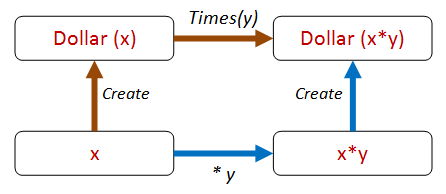
\includegraphics{pics/property_dollar_times.png}
\caption{Dollar times}
\end{figure}

Here's that property expressed in code:

\begin{minted}{fsharp}
let ``create then times should be same as times then create`` start 
    multiplier = 
        let d0 = Dollar.Create start
        let d1 = d0.Times(multiplier)
        let d2 = Dollar.Create (start * multiplier)     
        d1 = d2
\end{minted}
Great! Let's see if it works!

\begin{minted}{fsharp}
Check.Quick ``create then times should be same as times then create``
// Falsifiable, after 1 test
\end{minted}
Oops -- it doesn't work!
Why not? Because we forgot that \texttt{Dollar} is a reference type and
doesn't compare equal by default!
As a result of this mistake, we have discovered a property that we might
have overlooked! Let's encode that before we forget.

\begin{minted}{fsharp}
let ``dollars with same amount must be equal`` amount = 
	let d1 = Dollar.Create amount 
	let d2 = Dollar.Create amount 
	d1 = d2

Check.Quick ``dollars with same amount must be equal`` 
// Falsifiable, after 1 test
\end{minted}
So now we need to fix this by adding support for \texttt{IEquatable} and
so on.
You can do that if you like -- I'm going to switch to F\# record types
and get equality for free!

\subsection{Dollar properties -- version
3}\label{dollar-properties-version-3}

Here's the \texttt{Dollar} rewritten again:

\begin{minted}{fsharp}
type Dollar = {amount:int } 
	with 
	member this.Add add = 
		{amount = this.amount + add }
	member this.Times multiplier  = 
		{amount = this.amount * multiplier }
	static member Create amount  = 
		{amount=amount}
\end{minted}
And now our two properties are satisfied:

\begin{minted}{fsharp}
Check.Quick ``dollars with same amount must be equal`` 
// Ok, passed 100 tests.

Check.Quick ``create then times should be same as times then create``
// Ok, passed 100 tests.
\end{minted}
We can extend this approach for different paths. For example, we can
extract the amount and compare it directly, like this:
\begin{figure}[htbp]
\centering
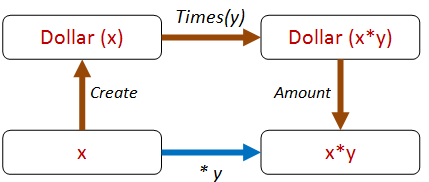
\includegraphics{pics/property_dollar_times2.png}
\caption{Dollar times}
\end{figure}
The code looks like this:

\begin{minted}{fsharp}
let ``create then times then get should be same as times`` start multiplier = 
	let d0 = Dollar.Create start
	let d1 = d0.Times(multiplier)
	let a1 = d1.amount
	let a2 = start * multiplier     
	a1 = a2

Check.Quick ``create then times then get should be same as times``
// Ok, passed 100 tests.
\end{minted}
And we can also include \texttt{Add} in the mix as well.

For example, we can do a \texttt{Times} followed by an \texttt{Add} via
two different paths, like this:

\begin{figure}[htbp]
\centering
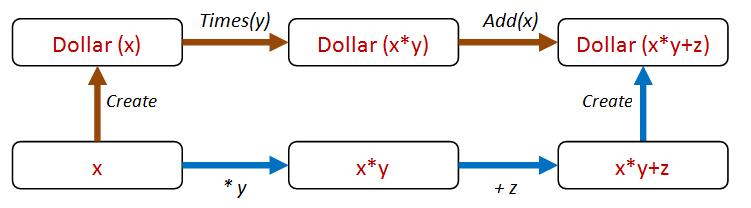
\includegraphics[width=0.95\textwidth]{pics/property_dollar_times3.png}
\caption{Dollar times}
\end{figure}

And here's the code:

\begin{minted}{fsharp}
let ``create then times then add should be same as times then add then 
    create`` start multiplier adder = 
        let d0 = Dollar.Create start
        let d1 = d0.Times(multiplier)
        let d2 = d1.Add(adder)
        let directAmount = (start * multiplier) + adder
        let d3 = Dollar.Create directAmount 
        d2 = d3

Check.Quick ``create then times then add should be same as times then 
    add then create`` 
// Ok, passed 100 tests.
\end{minted}
So this ``different paths, same result'' approach is very fruitful, and
we can generate \emph{lots} of paths this way.

\subsection{Dollar properties -- version
4}\label{dollar-properties-version-4}

Shall we call it done then? I would say not! 
We are beginning to get a whiff of a code smell. All this
\texttt{(start\ *\ multiplier)\ +\ adder} code seems like a bit of
duplicated logic, and could end up being brittle.

Can we abstract out some commonality that is present all these cases?
If we think about it, our logic is \emph{really} just this:

\begin{itemize}
\item
  Transform the amount on the ``inside'' in some way.
\item
  Transform the amount on the ``outside'' in the same way.
\item
  Make sure that the results are the same.
\end{itemize}

But to test this, the \texttt{Dollar} class is going to have to support
an arbitrary transform! Let's call it \texttt{Map}!
Now all our tests can be reduced to this one property:

\begin{figure}[htbp]
\centering
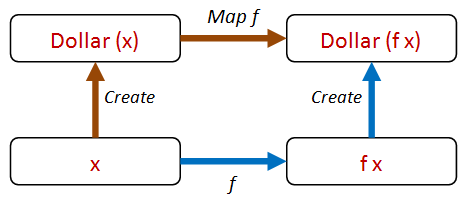
\includegraphics{pics/property_dollar_map.png}
\caption{Dollar map}
\end{figure}

Let's add a \texttt{Map} method to \texttt{Dollar}. And we can also
rewrite \texttt{Times} and \texttt{Add} in terms of \texttt{Map}:

\begin{minted}{fsharp}
type Dollar = {amount:int } 
	with 
	member this.Map f = 
		{amount = f this.amount}
	member this.Times multiplier = 
		this.Map (fun a -> a * multiplier)
	member this.Add adder = 
		this.Map (fun a -> a + adder)
	static member Create amount  = 
		{amount=amount}
\end{minted}
Now the code for our property looks like this:

\begin{minted}{fsharp}
let ``create then map should be same as map then create`` start f = 
	let d0 = Dollar.Create start
	let d1 = d0.Map f  
	let d2 = Dollar.Create (f start)     
	d1 = d2
\end{minted}
But how can we test it now? What functions should we pass in?
Don't worry! FsCheck has you covered! In cases like this, FsCheck will
actually generate random functions for you too!
Try it -- it just works!

\begin{minted}{fsharp}
Check.Quick ``create then map should be same as map then create`` 
// Ok, passed 100 tests.
\end{minted}
Our new ``map'' property is much more general than the original property
using ``times'', so we can eliminate the latter safely.

\subsection{Logging the function
parameter}\label{logging-the-function-parameter}

There's a little problem with the property as it stands. If you want to
see what the function is that FsCheck is generating, then Verbose mode
is not helpful.

\begin{minted}{fsharp}
Check.Verbose ``create then map should be same as map then create`` 
\end{minted}
Gives the output:

\begin{verbatim}
0:
18
<fun:Invoke@3000>
1:
7
<fun:Invoke@3000>
-- etc
98:
47
<fun:Invoke@3000>
99:
36
<fun:Invoke@3000>
Ok, passed 100 tests.
\end{verbatim}

We can't tell what the function values actually were.

However, you can tell FsCheck to show more useful information by
wrapping your function in a special \texttt{F} case, like this:

\begin{minted}{fsharp}
let ``create then map should be same as map then create2`` start (F (_,f)) = 
	let d0 = Dollar.Create start
	let d1 = d0.Map f  
	let d2 = Dollar.Create (f start)     
	d1 = d2
\end{minted}
And now when you use Verbose mode\ldots{}

\begin{minted}{fsharp}
Check.Verbose ``create then map should be same as map then create2`` 
\end{minted}
\ldots{} you get a detailed log of each function that was used:

\begin{verbatim}
0:
0
{ 0->1 }
1:
0
{ 0->0 }
2:
2
{ 2->-2 }
-- etc
98:
-5
{ -5->-52 }
99:
10
{ 10->28 }
Ok, passed 100 tests.
\end{verbatim}

Each \texttt{\{\ 2-\textgreater{}-2\ \}},
\texttt{\{\ 10-\textgreater{}28\ \}}, etc., represents the function that
was used for that iteration.


\section{TDD vs.~property-based
testing}\label{tdd-vs.property-based-testing}

How does property-based testing (PBT) fit in with TDD? This is a common
question, so let me quickly give you my take on it.

First off, TDD works with \emph{specific examples}, while PBT works with
\emph{universal properties}.

As I said in the previous post, I think examples are useful as a way
into a design, and can be a form of documentation. But in my opinion,
relying \emph{only} on example-based tests would be a mistake.

Property-based approaches have a number of advantages over example-based
tests:

\begin{itemize}
\item
  Property-based tests are more general, and thus are less brittle.
\item
  Property-based tests provide a better and more concise description of
  requirements than a bunch of examples.
\item
  As a consequence, one property-based test can replace many, many,
  example-based tests.
\item
  By generating random input, property-based tests often reveal issues
  that you have overlooked, such as dealing with nulls, missing data,
  divide by zero, negative numbers, etc.
\item
  Property-based tests force you to think.
\item
  Property-based tests force you to have a clean design.
\end{itemize}

These last two points are the most important for me. Programming is not
a matter of writing lines of code, it is about creating a design that
meets the requirements.
So, anything that helps you think deeply about the requirements and what
can go wrong should be a key tool in your personal toolbox!

For example, in the Roman Numeral section, we saw that accepting
\texttt{int} was a bad idea (the code broke!). We had a quick fix, but
really we should model the concept of a \texttt{PositiveInteger} in our
domain, and then change our code to use that type rather than just an
\texttt{int}. This demonstrates how using PBT can actually improve your
domain model, not just find bugs.

Similarly, introducing a \texttt{Map} method in the Dollar scenario not
only made testing easier, but actually improved the usefulness of the
Dollar ``api''.
Stepping back to look at the big picture, though, TDD and property-based
testing are not at all in conflict. They share the same goal of building
correct programs, and both are really more about design than coding
(think ``Test-driven \emph{design}'' rather than ``Test-driven
\emph{development}'').

\section{The end, at last}\label{the-end-at-last}

So that brings us to the end of another long post on property-based
testing! 
I hope that you now have some useful approaches that you can take away
and apply to your own code base.
Next time, we'll look at some real-world examples, and how you can
create custom generators that match your domain.

\emph{The code samples used in this post are
\href{https://github.com/swlaschin/PropertyBasedTesting/blob/master/part2.fsx}{available
on GitHub}}.
